\section{Forecasting}
Zaman serisi analizi, zaman içinde gözlenen verileri incelemek ve bu verilerin gelecekteki değerlerini tahmin etmek amacıyla istatistiksel ve veri madenciliği tekniklerinin uygulanmasıdır. Zaman serisi verileri, belirli bir zaman diliminde toplanan verileri temsil eder ve genellikle düzenli zaman aralıklarıyla gözlenir.

Zaman Serisi Modelleri: ARIMA (Oto-Regressif Entegre Hareketli Ortalama), GARCH (Genelleştirilmiş Oto-Regressif Koşullu Heteroskedastiklik), Exponential Smoothing (Üssel Düzleştirme)

\newpage

\subsection{Trend}
Trend, zaman içinde sürekli bir artış, azalış veya istikrarlı bir eğilimi ifade eder. Bu, bir zaman serisinin orta veya uzun vadeli değişimini temsil eder.

\subsubsection{Hareketli Ortalama (Moving Average)}

Zaman serisindeki gürültüyü azaltmak ve trendi yakalamak için hareketli ortalama yöntemi kullanılabilir. Basit bir hareketli ortalama veya ağırlıklı hareketli ortalama kullanılabilir.

\begin{lstlisting}[language=Python]
rolling_mean = time_series.rolling(window=10).mean()
\end{lstlisting}

\subsubsection{Lowess Düzleştirmesi (Locally Weighted Scatterplot Smoothing)}

Lowess düzleştirmesi, veriyi yumuşatarak ve yerel eğilimleri yakalayarak trendi belirlemek için kullanılır.

\begin{lstlisting}[language=Python]
from statsmodels.nonparametric.smoothers_lowess import lowess
smoothed = lowess(time_series, np.arange(len(time_series)), frac=0.2)
plt.figure(figsize=(12, 6))
plt.plot(time_series, label="Zaman Serisi")
plt.plot(smoothed[:, 0], label="Trend (Lowess Duzlestirmesi)", linestyle="--")
plt.xlabel("Zaman")
plt.ylabel("Deger")
plt.legend()
plt.grid(True)
plt.show()
\end{lstlisting}

\begin{figure}[h]
    \centering
    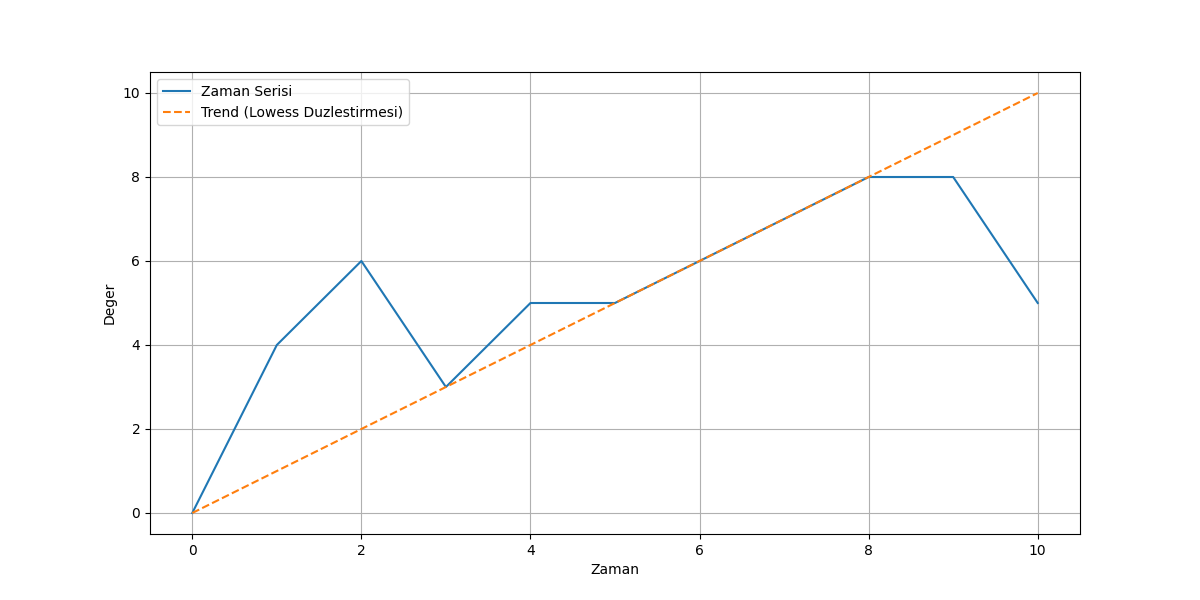
\includegraphics[width=0.6\textwidth]{images/lowess.png}
    \caption{Lowess düzleştirmesi örneği.}
    \label{fig:enter-label}
\end{figure}

\newpage

\subsection{Durağanlık (Stationary)}
Durağanlık, bir zaman serisinin istatistiksel özelliklerinin zaman içinde sabit olduğu veya dalgalanmadığı bir durumu ifade eder. Durağan bir zaman serisi, ortalama, varyans ve otokorelasyon gibi özellikler açısından zaman içinde tutarlıdır. 

\subsubsection{Augmented Dickey-Fuller (ADF) Testi}

Bir test, bir zaman serisinin birim kök (unit root) varlığını veya yokluğunu belirlemeye yardımcı olur. Birim kök, zaman serisinin durağanlık özelliği olmadığını ifade eder. ADF testi, null hipotezi H0 ve alternatif hipotezi H1; H0 = Zaman serisi birim kök içerir ve durağan değildir. H1 = Zaman serisi birim kök içermez ve durağandır.

\begin{lstlisting}[language=Python]
import pandas as pd
from statsmodels.tsa.stattools import adfuller

data = [10, 20, 30, 40, 50, 60, 70, 80, 90]
ts = pd.Series(data)

result = adfuller(ts)

print('ADF Istatistigi:', result[0])
print('p-degeri:', result[1])
print('Kritik degerler:', result[4])

if result[1] <= 0.05:
    print('Zaman serisi duragan.')
else:
    print('Zaman serisi duragan degil.')
\end{lstlisting}

\newpage

\subsubsection{Kwiatkowski-Philips-Schmidt-Shin (KPSS Testi)}

H0: Zaman serisi, düzgün (trend-stationary) durağanlık gösterir. H1: Zaman serisi, düzgün durağanlık göstermez (durağanlık göstermeyen birim kök içerir.). KPSS testi, genellikle iki farklı sürümde uygulanır: düzgün durağanlık testi (Level Stationary Test) ve trend durağanlık testi (Trend Stationary Test).

\begin{enumerate}
    \item Düzgün Durağanlık Testi (Level Stationary Test): H0: Zaman serisi düzgün durağanlık gösterir. H1: Zaman serisi düzgün durağanlık göstermez.
    \item Trend Durağanlık Testi (Trend Stationary Test): H0: Zaman serisi eğimli durağanlık gösterir. H1: Zaman serisi eğimli durağanlık göstermez.
\end{enumerate}

\begin{lstlisting}[language=Python]
from statsmodels.tsa.stattools import kpss

data = [10, 20, 30, 40, 50, 60, 70, 80, 90]
ts = pd.Series(data)

kpss_stat_level, p_value_level, lags_level, critical_values_level = kpss(ts, regression='c')

kpss_stat_trend, p_value_trend, lags_trend, critical_values_trend = kpss(ts, regression='ct')

print('Duzgun Duraganlik Test Istatistigi:', kpss_stat_level)
print('Duzgun Duraganlik Test p-degeri:', p_value_level)

print('Trend Duraganlik Test Istatistigi:', kpss_stat_trend)
print('Trend Duraganlik Test p-degeri:', p_value_trend)

if p_value_level <= 0.05:
    print('Zaman serisi duzgun duragan degil.')
else:
    print('Zaman serisi duzgun duragan.')

if p_value_trend <= 0.05:
    print('Zaman serisi trend duragan degil.')
else:
    print('Zaman serisi trend duragan.')
\end{lstlisting}

\newpage

\subsubsection{Philips-Perron Testi}

Zaman serisinin eğilimsiz (trend-stationary) durağanlık özelliğini değerlendirmek için kullanılır. H0: Zaman serisi eğilimsiz durağanlık gösterir. H1: Zaman serisi eğilimsiz durağanlık göstermez.

\begin{lstlisting}[language=Python]
from statsmodels.tsa.stattools import adfuller

data = [10, 20, 30, 40, 50, 60, 70, 80, 90]

ts = pd.Series(data)

result = adfuller(ts, regression='ct')

print('PP Istatistigi:', result[0])
print('p-degeri:', result[1])
print('Kritik degerler:', result[4])

if result[1] <= 0.05:
    print('Zaman serisi egilimsiz duragan.')
else:
    print('Zaman serisi egilimsiz duragan degil.')
\end{lstlisting}

\newpage

\subsubsection{Ljung-Box Testi}

Zaman serisinin otokorelasyonunu (kendi içindeki özbenzerliğini) test etmek için kullanılan bir istatistiksel testtir. Bu test, bir zaman serisinin rastgele gürültü içerip içeermediğini değerlendirmek amacıyla yaygın olarak kullanılır. Otokorelasyon, zaman serisinin kendisi ile belirli gecikmeler arasında pozitif veya negatif bir ilişki gösterip göstermediğini ölçer. H0: Zaman serisinin otokorelasyonu yoktur, yani zaman serisi bağımsızdır. H1: Zaman serisinde otokorelasyon vardır. Ljung-Box testi, belirli bir gecikme (lag) sayısı için bir test istatistiği hesaplar ve bu istatistiği karşılaştırılabilir bir eleştirel değerle karşılaştırır.

\begin{lstlisting}[language=Python]
from statsmodels.stats.diagnostic import acorr_ljungbox

data = [10, 20, 30, 40, 50, 60, 70, 80, 90]

ts = pd.Series(data)

lags = 5
lb_stat, p_value = acorr_ljungbox(ts, lags=lags)

print('Ljung-Box Istatistigi:', lb_stat)
print('p-degeri:', p_value)

if any(p_value <= 0.05):
    print('Zaman serisinde otokorelasyon vardir.')
else:
    print('Zaman serisinde otokorelasyon yoktur.')
\end{lstlisting}

\newpage

\subsection{Mevsimsel (Seasonal) Değişkenler}

Mevsimsel değişkenler, belirli bir dönemde, düzenli aralıklarla tekrar eden belirli bir deseni ifade eder. Mevsimsel değişkenler, zaman serisinin mevsimsel etkilerini veya desenlerini yakalamak için kullanılır.\\

\subsubsection{Aralık Tablosu (Seasonal Decomposition of TS - STL)}

Bu yöntem, zaman serisini trend, mevsimsel ve rastgele bileşenlere ayırmak için kullanılır.

\begin{lstlisting}[language=Python]
from statsmodels.tsa.seasonal import seasonal_decompose
result = seasonal_decompose(time_series, model='additive')
result.seasonal.plot()
\end{lstlisting}

\subsubsection{ACF (Autocorrelation Function) ve PACF (Partial Autocorrelation Function)}

\begin{lstlisting}[language=Python]
from statsmodels.graphics.tsaplots import plot_acf, plot_pacf
plot_acf(time_series, lags=50)
plot_pacf(time_series, lags=50)
\end{lstlisting}

\subsubsection{Differencing (Fark Alma)}

Zaman serisinde mevsimsel değişkenler varsa, veriyi fark alma (differencing) yöntemi kullanarak mevsimsel desenlerden arındırabilirsiniz. İlk fark, bir mevsimsel periyot boyunca (örneğin, bir yıl) yapılan farkı ifade eder. İkinci fark, ilk farkı fark alarak mevsimsel etkileri daha da azaltır.

\begin{lstlisting}[language=Python]
first_difference = time_series - time_series.shift(1)
second_difference = first_difference - first_difference.shift(1)
\end{lstlisting}

\subsubsection{Exponential Smoothing (Üstel Düzleştirme)}

Üstel düzleştirme yöntemleri (örneğin, Holt-Winters) mevsimsel değişkenleri modellemek için kullanılabilir. Bu yöntemler, verinin mevsimsel bileşenlerini ve mevsimsel desenlerini tahmin etmeye yardımcı olur.

\begin{lstlisting}[language=Python]
from statsmodels.tsa.holtwinters import ExponentialSmoothing
model = ExponentialSmoothing(time_series, seasonal='add', seasonal_periods=12)
result = model.fit()
seasonal_forecast = result.forecast(steps)
\end{lstlisting}

\subsubsection{Fourier Dönüşümleri}

Fourier dönüşümleri, mevsimsel desenleri modellendirmek için kullanılabilir. Bu yöntem, karmaşık mevsimsel desenleri yakalamak için sinüs ve kosinüs fonksiyonlarını kullanır.

\begin{lstlisting}[language=Python]
import numpy as np
import matplotlib.pyplot as plt
from scipy.fftpack import fft
t = np.linspace(0, 10, 1000) 
frequency = 0.2 
amplitude = 5
seasonal_component = amplitude * np.sin(2 * np.pi * frequency * t)
time_series = np.random.randn(1000) + seasonal_component
fourier_transform = fft(time_series)
magnitude = np.abs(fourier_transform)
seasonal_frequency = np.argmax(magnitude[1:]) / t[-1]
print(f"Mevsimsel frekans: {seasonal_frequency:.2f} periyot biriminde")
seasonal_component = amplitude * np.sin(2 * np.pi * seasonal_frequency * t)
non_seasonal_component = time_series - seasonal_component
plt.figure(figsize=(12, 6))
plt.plot(t, time_series, label="Mevsimsel Zaman Serisi")
plt.plot(t, seasonal_component, label="Mevsimsel Bilesen", linestyle="--")
plt.plot(t, non_seasonal_component, label="Mevsimsel Disi Bilesen", linestyle="--")
plt.xlabel("Zaman")
plt.ylabel("Deger")
plt.legend()
plt.grid(True)
plt.show()
\end{lstlisting}

\begin{figure}[h]
    \centering
    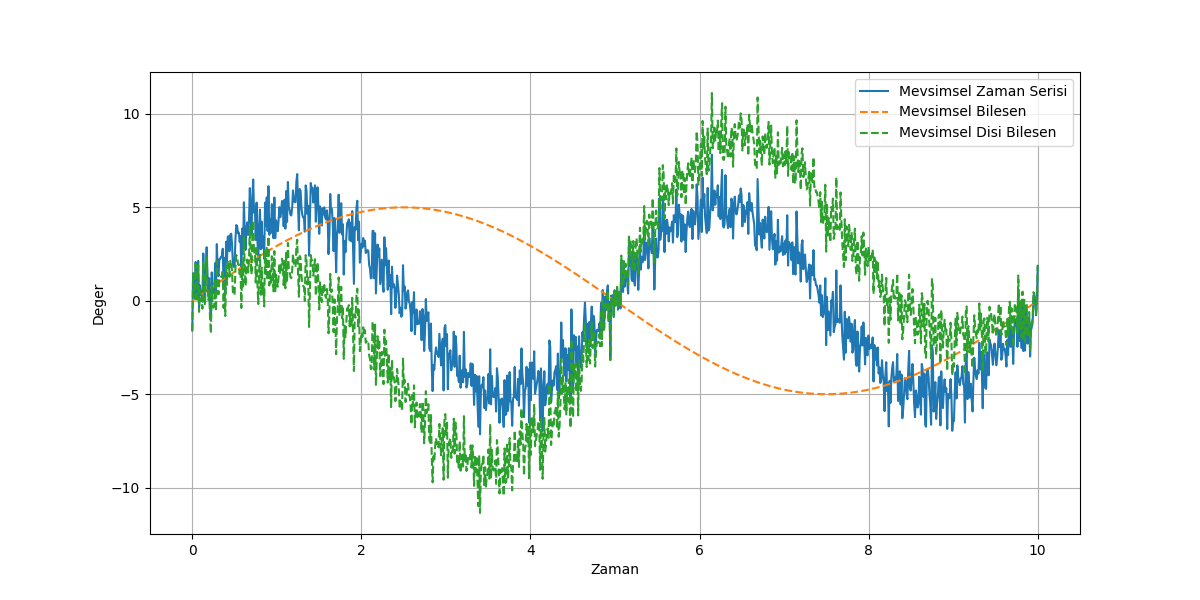
\includegraphics[width=0.7\textwidth]{images/fourier.png}
    \caption{Fourier dönüşümü örneği.}
    \label{fig:enter-label}
\end{figure}

\newpage

\subsection{Rastgele Gürültü (Noise)}
Rastgele gürültü, zaman serisindeki tahmin edilemeyen, rastgele veya stokastik dalgalanmalardır. Genellikle, trend ve mevsimsel desenlerin dışında kalan değişkenliklerin neden olduğu dalgalanmalar olarak düşünülür. Rastgele gürültü, zaman serisindeki diğer bileşenlerin modelleme ve tahmininde dikkate alınmaz.

\newpage